\chapter{Výsledky} % Ukazujeme co jsme zjistili
\label{ch:vysledky}
% Čistě výstupy práce — tabulky, grafy, hodnoty, klasifikační skóre, výpočty, srovnání metod atd.
% Popis, co se naměřilo, vypočítalo, co model vrátil atd., bez hlubší interpretace.
Tato kapitola obsahuje výsledky odhadu tepové frekvence z fotopletysmografických signálů pomocí tří různých metod:
referenčního Elgendiho algoritmu, vlastního algoritmu založeného na detekci systolických vrcholů a nově navržené metody využívající Hjorthovy deskriptory.

Výsledky jsou vyhodnoceny samostatně pro obě použité databáze: CapnoBase a \acl{BUT PPG}.
Výsledky automatického posouzení kvality signálů jsou shrnuty v~podkapitole~\ref{sec:vysledky_kvalita}.

%%%%%%%%%%%%%%%%%%%%%%%%%%%%%%%%%%%%%%%%%%%%%%%%%%%%%%%%%%%%%%%%%%%
%                            CapnoBase                            %
%%%%%%%%%%%%%%%%%%%%%%%%%%%%%%%%%%%%%%%%%%%%%%%%%%%%%%%%%%%%%%%%%%%
\section{Výsledky pro databázi CapnoBase}
\label{sec:vysledky_capnobase}
% Popsat statistické metody, které jsme použili pro vyhodnocení kvality detekce vrcholů.
% Tabulka s metrikama
% Signál se pro tuto databázi nepodvzorkovává, ale máme původních 300 Hz.
% Fun fact = výsledky Hjortha je pro podvzorkované signály HORŠÍ
U této databáze máme k dispozici referenční hodnoty systolických vrcholů, a proto můžeme použít statistické metody pro vyhodnocení kvality detekce, jako je citlivost (\acs{Se}), pozitivní prediktivní hodnota (\acs{PPV}) a F1 skóre.
Citlivost vyjadřuje procento vrcholů, které použitý algoritmus správně rozpoznal z celkového počtu \textit{referenčních} vrcholů:
\begin{equation}
	\label{eq:se}
	\acs{Se} = \frac{\acs{TP}}{\acs{TP} + \acs{FN}} \cdot 100\%.
\end{equation}
Vyšší citlivost znamená nižší riziko, že algoritmus opomene detekovat skutečný vrchol.

Pozitivní prediktivní hodnota vyjadřuje procento vrcholů, které vybraný algoritmus určil správně z celkového počtu \textit{detekovaných} vrcholů:
\begin{equation}
	\label{eq:ppv}
	\acs{PPV} = \frac{\acs{TP}}{\acs{TP} + \acs{FP}} \cdot 100\%.
\end{equation}
Vyšší hodnota \acs{PPV} znamená, že algoritmus detekuje méně falešných vrcholů.

\acs{F1} skóre je harmonický průměr citlivosti a \acs{PPV} vyjádřen v procentech:
\begin{equation}
	\label{eq:f1}
	\acs{F1} = 2 \cdot \frac{Se \cdot PPV}{Se + PPV} \cdot 100\%.
\end{equation}

Tyto metriky počítáme pouze pro Elgendiho algoritmus a vlastní algoritmus detekce vrcholů, kvůli povaze algoritmu využívajícího Hjorthovu mobilitu, který neprovádí detekci vrcholů, ale přímo odhaduje tepovou frekvenci.
Když jsme je ale počítali, nastavili jsme toleranční pásmo pro výpočet matice záměn na $\pm$0,1~\acs{s}, které nám definuje, jak daleko od referenčního vrcholu se může detekovaný vrchol nacházet, aby byl považován za správně detekovaný.
V~Tab.~\ref{tab:capnobase_comparison} jsou hodnoty \acs{Se} a \acs{PPV} vypočítány ze součtu všech \acs{TP}, \acs{FP} a \acs{FN}.
\acs{F1} skóre je pak vypočítáno z těchto hodnot.

Dále jsme vyhodnotili průměrnou absolutní chybu (\acs{MAE}) mezi referenční a odhadovanou tepovou frekvencí dle rovnice~(\ref{eq:mae}).

\begin{equation}
	\label{eq:mae}
	\acs{MAE} = \frac{1}{N} \sum_{i=1}^{N} |TF_{i,ref} - TF_{i,est}|
\end{equation}

Jako dodatečné kritérium jsme stanovili poměr mezi dobře a špatně odhadnutými signály.
Za dobře odhadnuté byly považovány signály s \acs{MAE} menší než 5~\acs{bpm}, což odpovídá prahové hodnotě dle mezinárodního standardu IEC~60601-2-27 a metodice databáze \acs{BUT PPG}~\cite{BUT_PPG}.
V tabuce používáme označení \uv{d:š} pro poměr \uv{dobře:špatně} odhadnutých signálů.
% Po vypočítání průměrné kvadratické chyby (\acs{RMSE})~(\ref{eq:rmse}) mezi referenční a odhadovanou \acs{TF} jsme nastavili prahovou hodnotu \acs{RMSE} na XX tepů za minutu.

Poslední sledovanou metrikou byla výpočetní náročnost jednotlivých algoritmů, vyjádřená jako celkový čas potřebný ke zpracování celé databáze CapnoBase.
Výpočty probíhaly na platformě Apple M1.
Hodnoty jsou orientační a slouží pouze k vzájemnému srovnání mezi algoritmy.
Vzhledem k rozdílným charakteristikám databází (odlišná vzorkovací frekvence, délka i počet signálů, datový formát) nejsou časy mezi CapnoBase a \acs{BUT PPG} přímo srovnatelné.

Metriky přesnosti pro všechny tři algoritmy jsou uvedeny v~Tab.~\ref{tab:capnobase_comparison}, a to vždy pro různé délky vstupního signálu.

% table with comparison of methods
\begin{table}[!ht]
	\centering
	\caption[Srovnání metod odhadu TF na databázi CapnoBase]{Srovnání metod odhadu TF.}
	\label{tab:capnobase_comparison}
	\resizebox{\textwidth}{!}{
		\begin{tabular}{|l|c|c|c|c|c|c|}
			\hline
			\textbf{                  } &  \textbf{Se}  &  \textbf{PPV} &  \textbf{F1}  &     \textbf{MAE}     & \textbf{Poměr} & \textbf{Čas} \\
			\textbf{Metoda} (délka [s]) & \textbf{[\%]} & \textbf{[\%]} & \textbf{[\%]} & \textbf{[\acs{bpm}]} & \textbf{[d:š]} & \textbf{[s]} \\
			\hline\hline
			Elgendi (480)        & 99,81 & 99,89 & 99,85 & 0,31 &   42:0   &  16,1 \\
			\hline
			Elgendi (62,5)       & 99,23 & 99,88 & 99,55 & 0,35 &   336:0  &  17,9 \\
			\hline
			Vlastní vrcholová    & 99,34 & 99,91 & 99,63 & 0,31 &   42:0   &  2,4  \\
			detekce (480)        &       &       &       &      &          &       \\
			\hline
			Vlastní vrcholová    & 98,49 & 99,91 & 99,20 & 0,37 &   336:0  &  2,7  \\
			detekce (62,5)       &       &       &       &      &          &       \\
			\hline
			Hjorth (480)         &  --   &  --   &  --   & 1,52 &   40:2   &  2,6  \\
			\hline
			Hjorth (60)          &  --   &  --   &  --   & 0,80 &   332:4  &  2,7  \\
			\hline
			Hjorth (10)          &  --   &  --   &  --   & 0,61 &  2015:1  &  14,5 \\
			\hline
		\end{tabular}
		}
\end{table}

Na Obr.~\ref{fig:capnobase_SePPV_1min} a~Obr.~\ref{fig:capnobase_SePPV_8min} je znázorněno srovnání citlivosti a~přesnosti mezi vlastní metodou detekce vrcholů a~referenční Elgendiho metodou.
První obrázek zobrazuje výsledky pro minutové úseky (přeněji 62,5~s), zatímco druhý shrnuje výstupy pro celé osmiminutové záznamy.
Nejnižší hodnotu citlivosti vykazuje náš algoritmus ve druhé minutě signálu 0115, což odpovídá případu zobrazenému na Obr.~\ref{fig:capnobase_our_err}.

\begin{figure}[!ht]
	\centering
	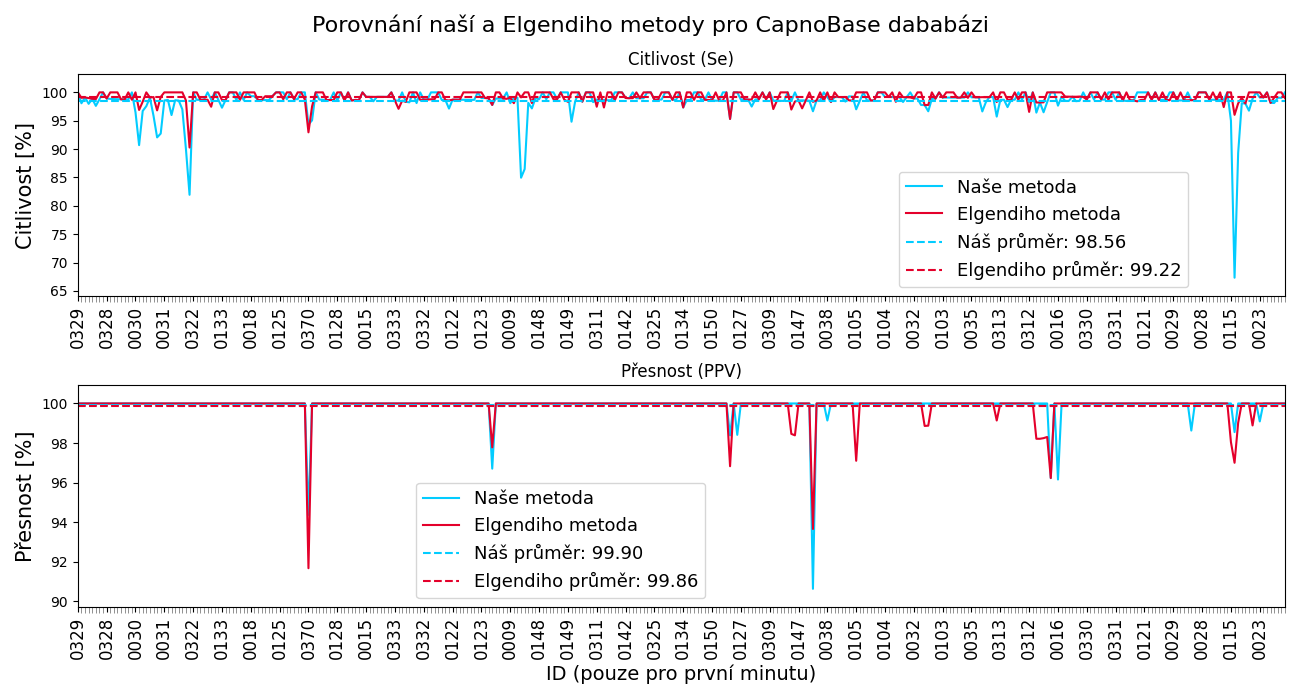
\includegraphics[width=1\textwidth]{./obrazky/vysledky/CB_Elgendi_Our_chunked.png}
	\caption[Srovnání metod detekující vrcholy pro minutové úseky]{Srovnání metod detekující vrcholy pro minutové úseky.}
	\label{fig:capnobase_SePPV_1min}
\end{figure}

\begin{figure}[!ht]
	\centering
	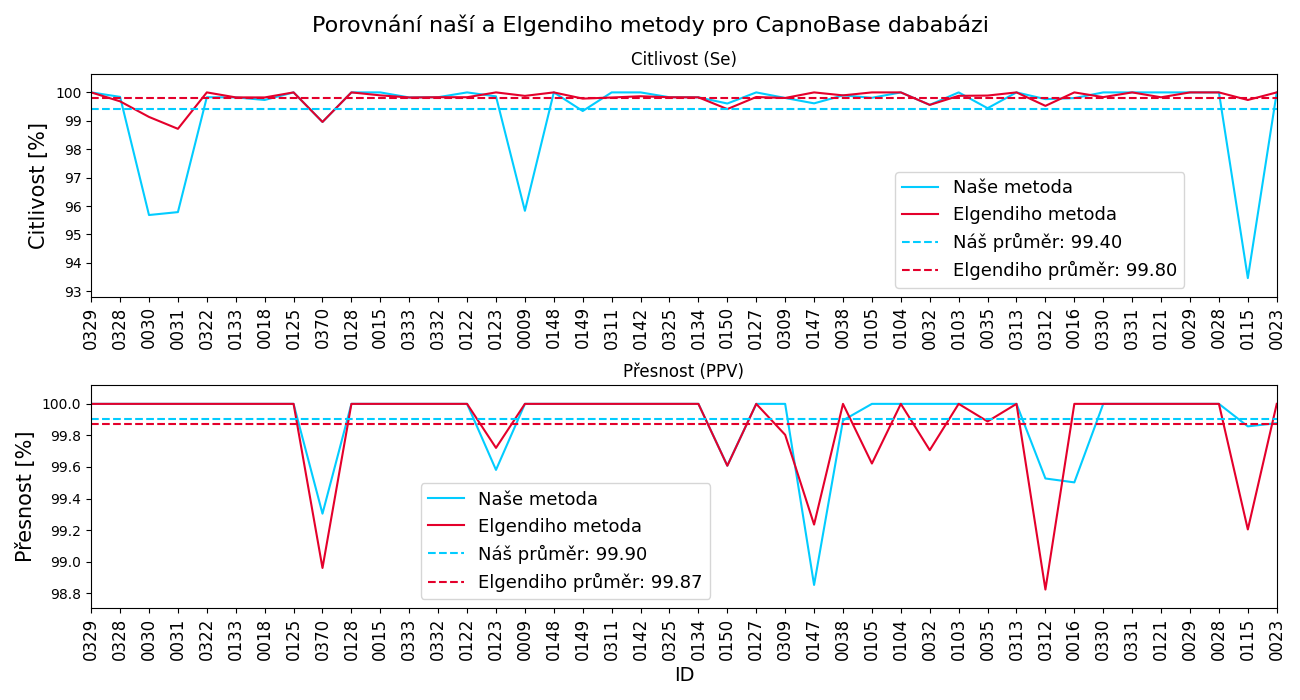
\includegraphics[width=1\textwidth]{./obrazky/vysledky/CB_Elgendi_Our_full.png}
	\caption[Srovnání metod detekující vrcholy pro celý signál]{Srovnání metod detekující vrcholy celý signál.}
	\label{fig:capnobase_SePPV_8min}
\end{figure}

\begin{figure}[!ht]
	\centering
	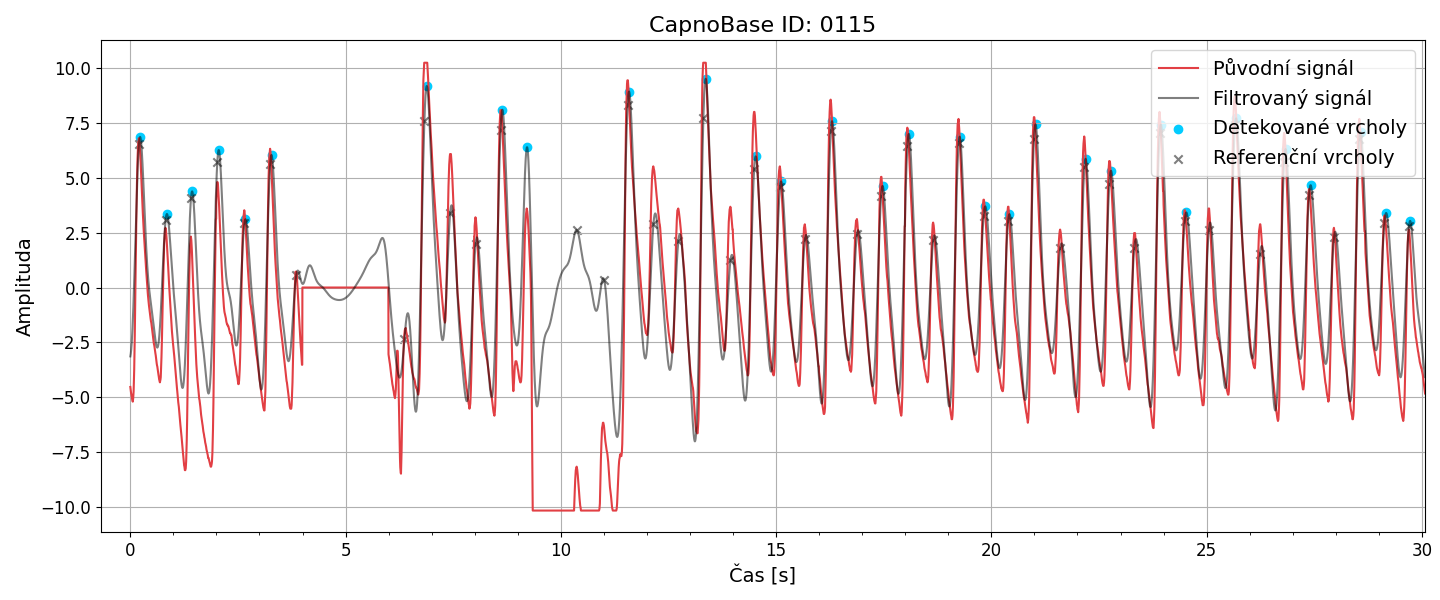
\includegraphics[width=0.9\textwidth]{./obrazky/vysledky/CB_Our_err.png}
	\caption[Chybný odhad \acs{TF} pomocí vlastní vrcholové detekce]{Chybný odhad TF pomocí vlastní vrcholové detekce.}
	\label{fig:capnobase_our_err}
\end{figure}

Je důležité poznamenat, že zobrazené hodnoty \acs{Se} a~\acs{PPV} se v~grafech liší od hodnot uvedených v~Tab.~\ref{tab:capnobase_comparison}.
V tabulce jsou hodnoty vypočteny jako agregovaná hodnota pro celou databází (tj. globální součet všech \acs{TP}, \acs{FP} a~\acs{FN})
Na druhou stranu, v~grafech jsou vypočítané hodnoty \acs{Se} a~\acs{PPV} individuálně a~z~těch je následně vypočítán a vykreslen průměr.
Tento přístup lépe odpovídá srovnání výkonnosti napříč jednotlivými záznamy, zatímco tabulková metrika lépe charakterizuje celkový výkon algoritmů.

Bland-Altmanovy grafy znázorněné na Obr.~\ref{fig:capnobase_BlandAltman_peaks} porovnávají rozdíl mezi odhadovanou a~referenční tepovou frekvencí pro obě metody detekce vrcholů.
Výsledky jsou rozděleny nejen podle použité metody (vlastní versus Elgendi), ale také podle délky analyzovaných úseků -- zvlášť pro celé osmiminutové signály a zvlášť pro jejich 62,5~s dlouhé úseky.
V grafech jsou vyznačeny průměrné odchylky (\acs{ME}) jako zelená přerušovaná čára, zatímco hranice shody, definované jako $\pm1,96 \cdot \acs{SD}$, jsou znázorněny červenými přerušovanými čarami.
Tato rozdílová analýza umožňuje posoudit, jak výrazně se odhady liší od referenčních hodnot a zda je chyba závislá na velikosti tepové frekvence.

\begin{figure}[!bh]
	\centering
	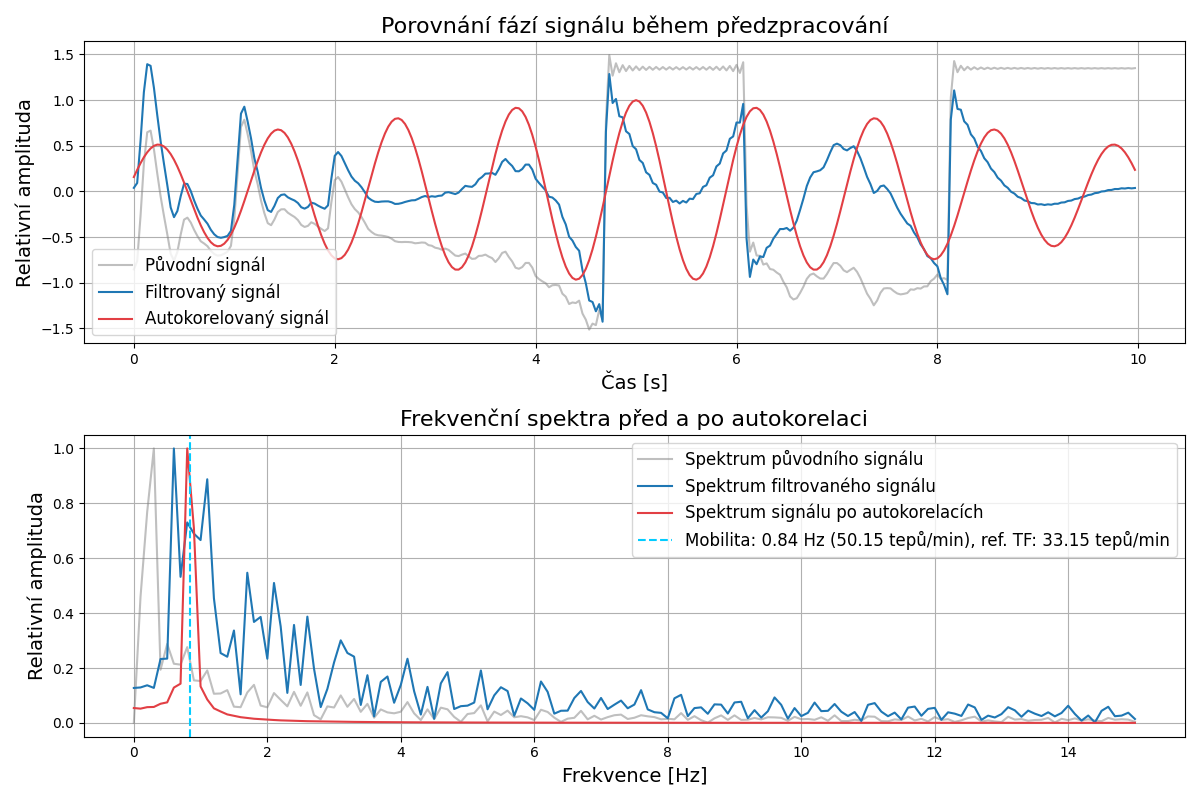
\includegraphics[width=0.9\textwidth]{./obrazky/vysledky/hjorth_preprocess_diffHR.png}
	\caption[Chybný odhad \acs{TF} pomocí Hjorthových deskriptorů u nekvalitního signálu]{Chybný odhad TF pomocí Hjorthových deskriptorů u nekvalitního signálu.}
	\label{fig:capnobase_hjorth_err}
\end{figure}

Obr.~\ref{fig:capnobase_BlandAltman_hjorth} zachycuje výsledky Bland-Altmanovy analýzy pro metodu využívající Hjorthovy deskriptory.
Grafy jsou opět rozděleny dle délky analyzovaných úseků: horní pro celé signály, prostřední pro minutové segmenty a spodní pro desetisekundové úseky.
V posledním grafu byly zahrnuty pouze signály označené jako kvalitní, čímž byl vyloučen jeden extrémně odlehlý případ (signál 0147, 25. minuta), který by vzhledem ke své vysoké chybě narušil škálu zobrazení.
Tento úsek je detailně zachycen na Obr.~\ref{fig:capnobase_hjorth_err}, kde je patrná výrazná deformace signálu a posun dominantní frekvence.
Společně s ním bylo vyloučeno dalších 15 signálů.

\begin{figure}[!ht]
	\centering
	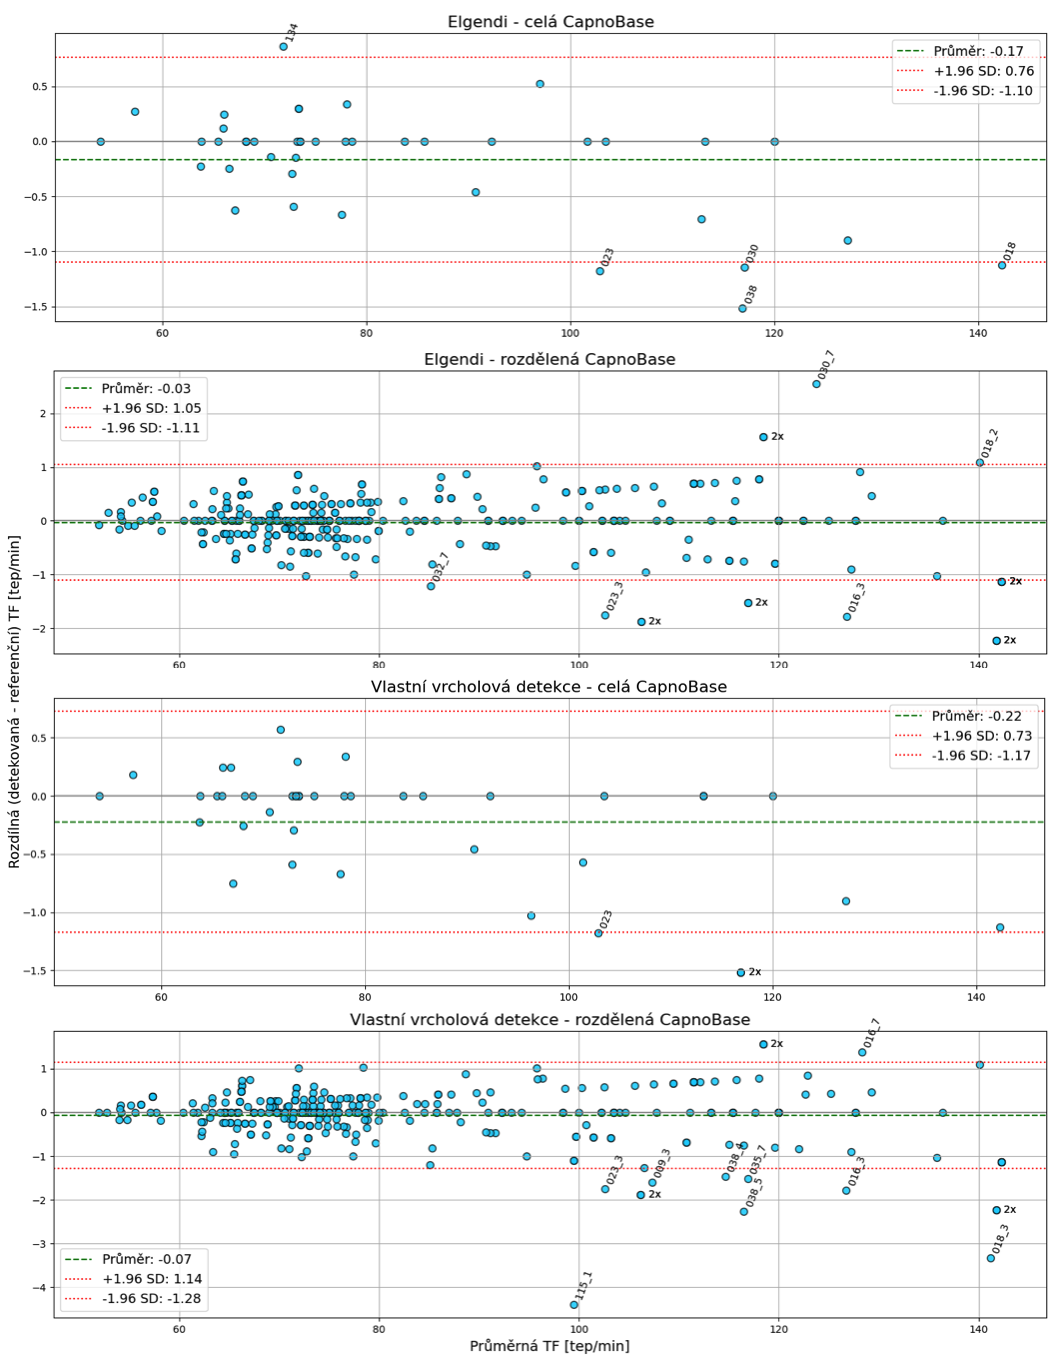
\includegraphics[width=1\textwidth]{./obrazky/vysledky/BlandAltman_CB_peaks.png}
	\caption[Bland-Altmanova analýza pro metody detekující vrcholy - CapnoBase]{Bland-Altmanova analýza pro metody detekující vrcholy.}
	% \vspace{-10mm}
	\label{fig:capnobase_BlandAltman_peaks}
\end{figure}

\begin{figure}[!ht]
	\centering
	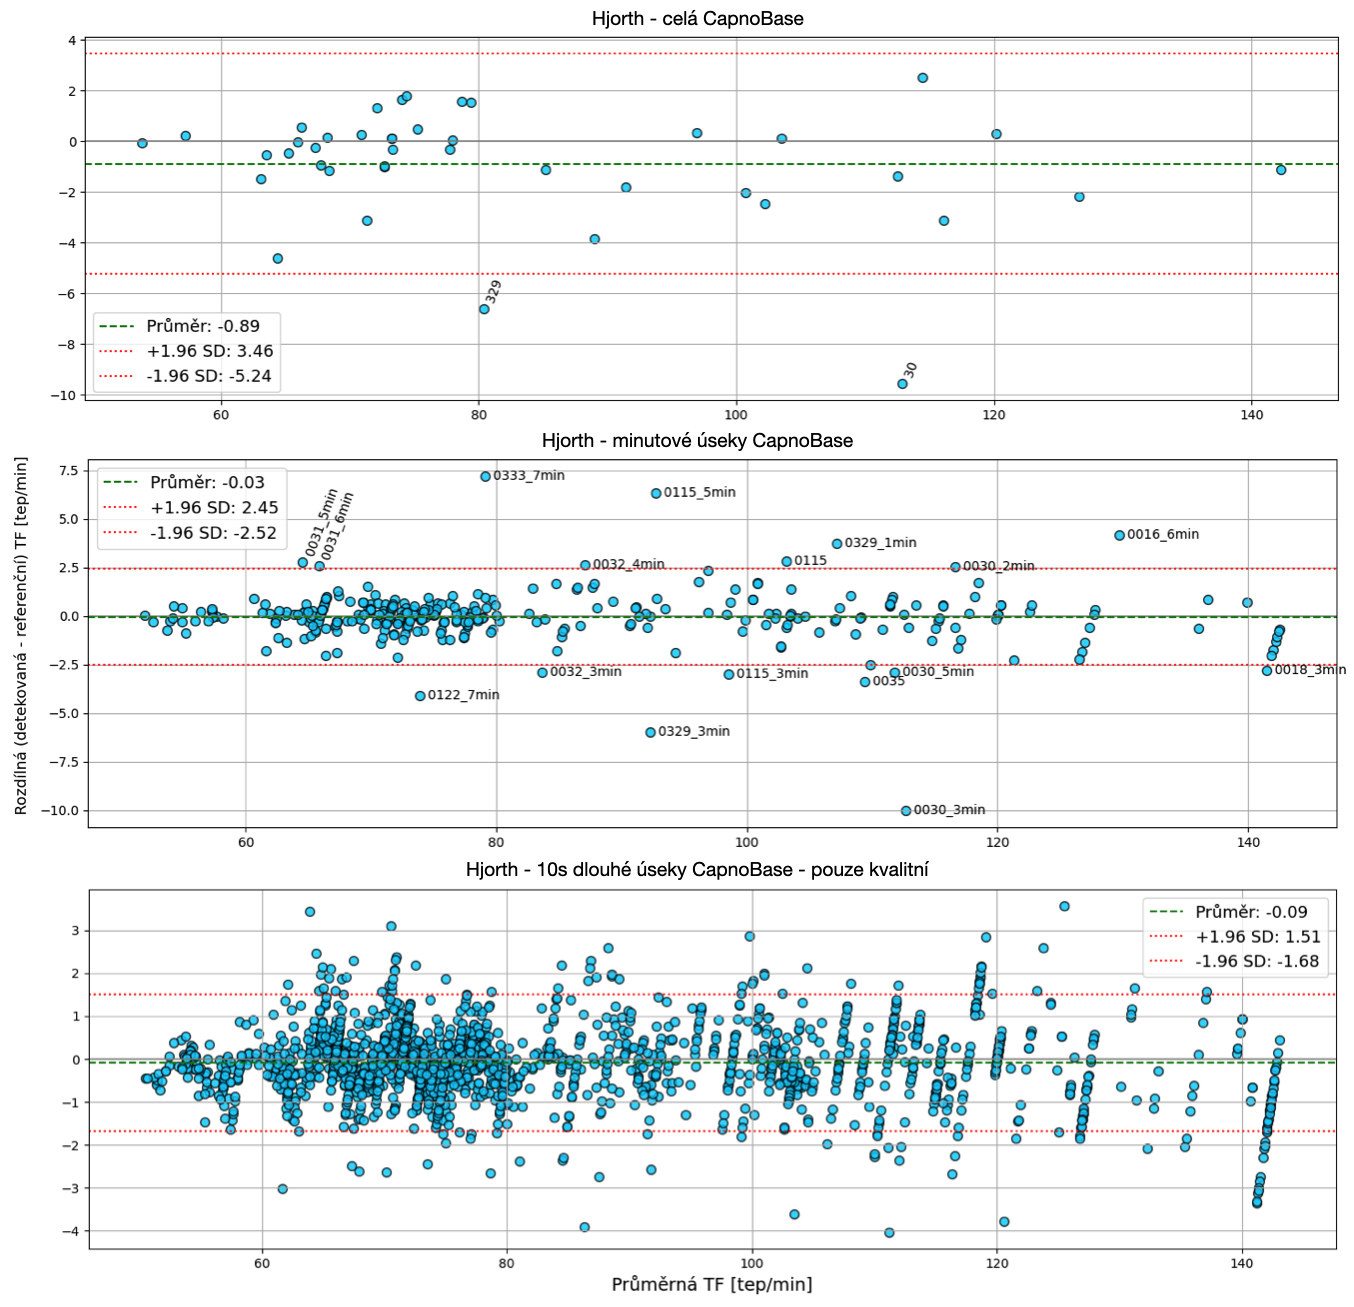
\includegraphics[width=1\textwidth]{./obrazky/vysledky/BlandAltman_CB_Hjorth.png}
	\caption[Bland-Altmanova analýza pro metodu využívající Hjorthovy deskriptory - CapnoBase]{Bland-Altmanova analýza pro metodu využívající Hjorthovy deskriptory.}
	\label{fig:capnobase_BlandAltman_hjorth}
\end{figure}

%%%%%%%%%%%%%%%%%%%%%%%%%%%%%%%%%%%%%%%%%%%%%%%%%%%%%%%%%%%%%%%%%%%
%                             BUT PPG                             %
%%%%%%%%%%%%%%%%%%%%%%%%%%%%%%%%%%%%%%%%%%%%%%%%%%%%%%%%%%%%%%%%%%%
\FloatBarrier
\section{Výsledky pro databázi BUT PPG}
\label{sec:vysledky_butppg}
% Popsat jaké metriky jsme použili pro vyhodnocení kvality detekce TF - už nedetekujeme vrcholy.
Databáze \acs{BUT PPG} neobsahuje referenční anotace systolických vrcholů, a není proto možné vyhodnotit metriky citlivosti (\acs{Se}), přesnosti (\acs{PPV}) ani F1 skóre.
Pro posouzení výkonu jednotlivých algoritmů při odhadu tepové frekvence jsme proto použili průměrnou absolutní chybu (\acs{MAE}) definovanou rovnicí~(\ref{eq:mae}).
Za správně odhadnuté byly považovány ty signály, u nichž byla \acs{MAE} menší než 5~\acs{bpm}, tedy ve shodě s prahovou hodnotou použité již v předchozí podkapitole a doporučenou dle normy IEC~60601-2-27.

Jelikož se v databázi nachází značný počet nekvalitních signálů, byly výsledky interpretovány s ohledem na kvalitu vstupních dat.
K tomu byly využity dvě hodnoty: původní, referenční skóre \acs{R-SQI}, přítomné v metadatech databáze, a dále skóre \acs{O-SQI} získané pomocí algoritmu podle Orphanidou, detailněji popisovaného v~podkapitole~\ref{subsec:referencni_hodnota_kvality}.
Obě hodnoty umožňují binárně rozdělit signály na kvalitní a nekvalitní, což následně slouží k oddělenému hodnocení přesnosti odhadů \acs{TF}.

Souhrnné výsledky pro všechny tři metody odhadu \acs{TF} jsou uvedeny v Tab.~\ref{tab:but_ppg_comparison}.
Výsledky jsou prezentovány ve třech scénářích: pro celou databázi, pro signály označené jako kvalitní na základě \acs{R-SQI} a pro kvalitní signály dle \acs{O-SQI}.
Podobně jako u vyhodnocení databáze CapnoBase jsou kromě hodnoty \acs{MAE} uvedeny také poměry dobře a špatně odhadnutých tepových frekvencí a orientační výpočetní čas algoritmů.

\begin{table}[!ht]
	\centering
	\caption[Srovnání metod odhadu TF na databázi BUT PPG]{Srovnání metod odhadu TF.}
	\label{tab:but_ppg_comparison}
	\resizebox{\textwidth}{!}{
		\begin{tabular}{|l|c|c||c|c||c|c||c|}
			\hline
			\textbf{       } & \multicolumn{2}{|c|}{\textbf{celá databáze}} & \multicolumn{2}{|c|}{\textbf{\acs{R-SQI}}}  & \multicolumn{2}{|c|}{\textbf{\acs{O-SQI}}} &  \\
			\hline
			\textbf{       } &     \textbf{MAE}     & \textbf{Poměr} &     \textbf{MAE}     & \textbf{Poměr} &     \textbf{MAE}     & \textbf{Poměr} & \textbf{Čas} \\
			\textbf{Metoda}  & \textbf{[\acs{bpm}]} & \textbf{[d:š]} & \textbf{[\acs{bpm}]} & \textbf{[d:š]} & \textbf{[\acs{bpm}]} & \textbf{[d:š]} & \textbf{[s]} \\
			\hline\hline
			Elgendi          &  18,84  & 875\textbf{:}2.797 &  6,73   &  511\textbf{:}299  &  7,82  &  177\textbf{:}90  &  x  \\
			\hline
			Vlastní          &         &                    &         &                    &        &                   &     \\
			vrcholová        &  20,54  & 875\textbf{:}2.797 &  7,80   &  507\textbf{:}303  &  7,12  &  183\textbf{:}84  &  x  \\
			detekce          &         &                    &         &                    &        &                   &     \\
			\hline
			Hjorth           &  31,22  & 624\textbf{:}3.048 &  12,98  &  497\textbf{:}313  &  8,05  &  182\textbf{:}85  &  x  \\
			\hline
		\end{tabular}
		}
\end{table}

\begin{figure}[!ht]
	\centering
	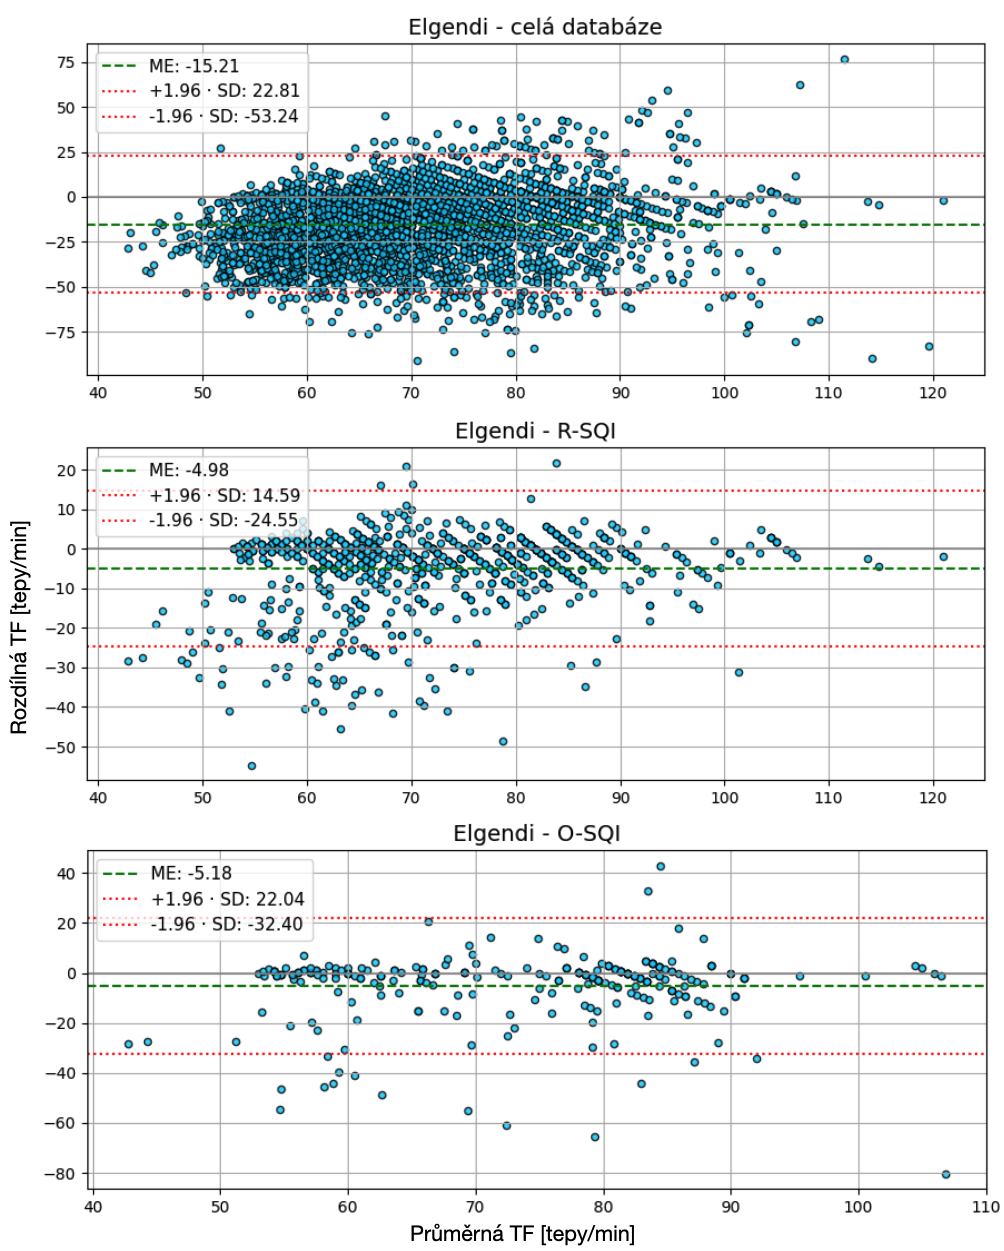
\includegraphics[width=1\textwidth]{./obrazky/vysledky/BA_BUT_Elgendi.png}
	\caption[Bland-Altmanova analýza pro Elgendiho metodu - BUT PPG]{Bland-Altmanova analýza pro Elgendiho metodu.}
	\label{fig:BUT_BlandAltman_elgendi}
\end{figure}

\begin{figure}[!ht]
	\centering
	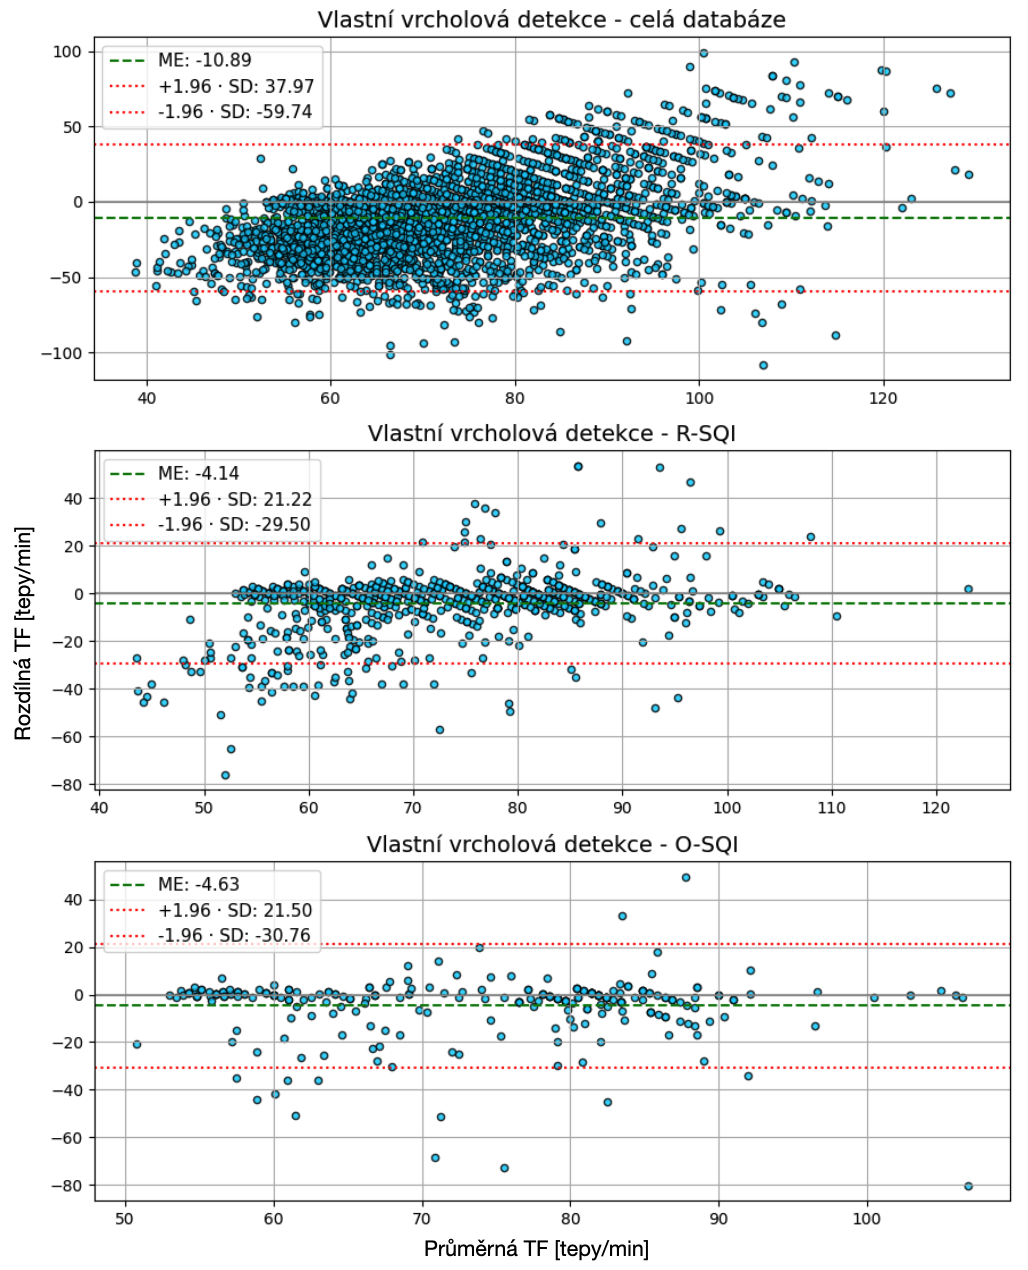
\includegraphics[width=1\textwidth]{./obrazky/vysledky/BA_BUT_VVD.png}
	\caption[Bland-Altmanova analýza pro naši metodu detekující vrcholy - BUT PPG]{Bland-Altmanova analýza pro naši metodu detekující vrcholy.}
	\label{fig:BUT_BlandAltman_vvd}
\end{figure}

\begin{figure}[!ht]
	\centering
	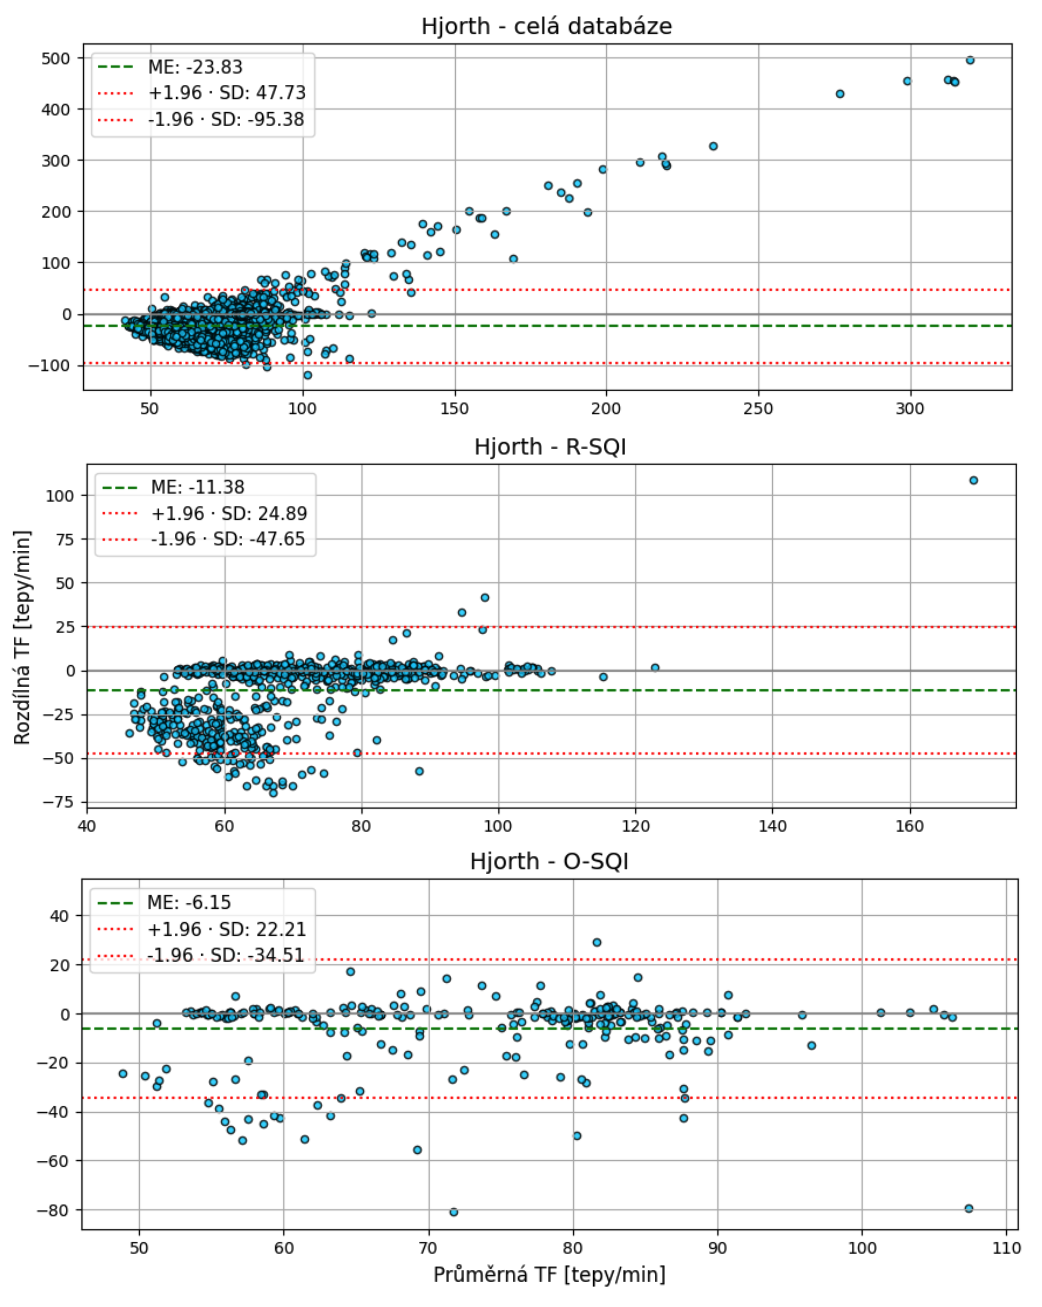
\includegraphics[width=1\textwidth]{./obrazky/vysledky/BA_BUT_Hjorth.png}
	\caption[Bland-Altmanova analýza pro metodu využívající Hjorthovy deskriptory - BUT PPG]{Bland-Altmanova analýza pro metodu využívající Hjorthovy deskriptory.}
	\label{fig:BUT_BlandAltman_hjorth}
\end{figure}

%%%%%%%%%%%%%%%%%%%%%%%%%%%%%%%%%%%%%%%%%%%%%%%%%%%%%%%%%%%%%%%%%%%
%                             Kvalita                             %
%%%%%%%%%%%%%%%%%%%%%%%%%%%%%%%%%%%%%%%%%%%%%%%%%%%%%%%%%%%%%%%%%%%
\FloatBarrier
\section{Výsledky automatického posouzení kvality}
\label{sec:vysledky_kvalita}